\documentclass[12pt]{standalone}


\usepackage{amssymb} 
\usepackage{amsmath} 

\usepackage[no-math]{fontspec}
\usepackage{unicode-math}
\setmainfont{TeX Gyre Heros}
\setmathfont{Stix Two Math}

\usepackage{tikz}
\usetikzlibrary{arrows.meta, backgrounds}

\usepackage{xcolor}
\definecolor{bgcolor}{HTML}{F3F4F4}

\begin{document}
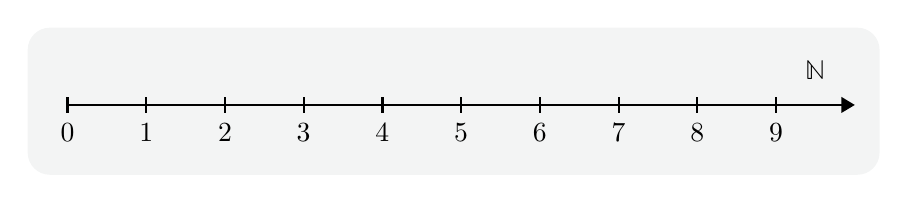
\begin{tikzpicture}[
    show background rectangle,
    background rectangle/.style={fill=bgcolor, rounded corners=8pt},
    inner frame sep=0.3cm
]
  % Draw the main line with arrow on the right
  \draw[thick, -{Triangle}] (0,0) -- (10,0);
  
  % Draw tick marks and labels
  \foreach \x in {0,1,2,3,4,5,6,7,8,9} {
    \draw[thick](\x,0.1) -- (\x,-0.1);
    \node[below] at (\x,-0.1) {\x};
  }
  
  % Optional: Add a label for the number line
  \node[above] at (9.5,0.2) {$\mathbb{N}$};
\end{tikzpicture}
\end{document}